\section{Evaluation}\label{sec:eval}
%
%\struc{small introduction sentence to this section}
The following subsections will primarily focus on visualizing and analyzing the key metrics we collect for each proxy- and mini-app,
such as \unit[]{Gflop/s}. The significance of our findings with respect to future software, CPU, and HPC system design will then
be discussed in the next Section~\ref{sec:discuss}.
%High or low \unit[]{operations/s}, see Section~\ref{ssec:eval_ops} and~\ref{ssec:eval_flops}, or \unit[]{byte/s}, see
%Section~\ref{ssec:eval_mem}, by itself is not a good indication about the system's bottlenecks\cJD{This full sentence is ambiguous}.
Analyzing the instruction mix, \unit[]{flop/s}, or memory throughput,
see Section~\ref{ssec:eval_ops},~\ref{ssec:eval_flops}, and~\ref{ssec:eval_mem},
in a isolated fashion is not a good indication about the system's bottlenecks,
and hence, especially when reasoning about FPU requirements, we also have to understand
the applications' compute-boundedness, which we evaluate in Section~\ref{ssec:eval_freq}.
Table~\ref{tb:Mtools} summarizes the primary metrics and method/tool to collect these metrics. Table~\ref{table:rest} includes additional metrics. 
%\struc{which metrics are we collecting, how is each collected, and/or derived from other metrics, and most importantly: why do we care about this metric; add formulae if necessary}
%\struc{need at least: FP ratio, Int, freq scaling, memory BW, ...TBA}
%\cJD{have to analzye the run2run variation among the 10 speed runs} done that
%

% goal: 2.5 -- 3 pages
% language (report) + program desciption + (Minami-san classication M1-M6 or so for apps)
% run time overall (can measure but not strickly needed)
% time in solver
% abs numbers / percentage instructions
% performance in (sp/dp) gflop/s
% total #flops (part of 2. above)
% memory usage (peak mem util ; memory throughput; info from vtune?? for L1/L2/L3?) -> try carefully vtune
% !! fix uncore to max.
% !! KNL+KNM keep at max freq. (perf govenour + max fequ)
% resource stall counter (abs/percentage) -> vtune
% LLC hit/miss rate (also +L2 rates if in mcdram in cache; skip flat mode)
% fp64/fp32/int/(branch?)/(unconditional memory ops; -> LOAD/STORE) instructions -> get load/store from SDE (ask artur for details)
% power usage (use pcm-power and report per kernel number)
% memory-boundness, multitude of tests based on, and list all:
%  - educated guess + flops/to/bytes
%  - roof line (!skip)
%  - stalled instructions (artur: diff from resource stall counter)
%  - frequ. scaling -> least important item (skip if not needed)
%  - mcdram? vs ddr? (skip flat mode but report that we tried -> faster memory -> faster exec?)
%  - traffic betw. LLC and RAM (pcm-mem and CAREFUL about broken numbers on socket 1 on kiev)
%  (-- how much does each of these contribute to the ground-truth???)
% normalized based on number of core or absolute numbers, dep. on context/what to show
% ** create all graphs and check for the **anomalies**
%
% => all 3 systems (find kiev w/ right pcm results)
%
% put uninteresting stuff into TechReport
%
%% BM list
%
%  - memory foot print (ignore KNM because heaptrack broken -> but use lyon numbers to extrapolate)
%  - running scripts: jens has all
%  - scipts for  analysin g results : matsumura
%  - script for figure creating : matsumura
%  - master script: jens
%  - FORCED blackout aug! ->careful when to run
%  - solo on system (init 3?); any OS variance? SAME kernel! -> avoid the one with gnome (maybe lyon3+mill1+kiev5) -> maybe 3 ssd or ask nomura what best to isolate node (init 3 plus network stack maybe)
%  - take best time and recalculate mem throughput / power reported based on best time and not based on time in the run of pcm (if vastly different)
%
%matsumura: memory used on ngsa? heaptrack -> broken?
%matsumura: what is "copy of ..." sheets? flat or cache?
%yashima: KNL numbers updated for SW4lite: forgot to update colors or no yet updated?
%artur: powsample: reports processor or cpu+mem? we see 234W in one app on KNL whihc is above TDP (230W)
%jens: pcm-pwer: main result is cpu or node??? -> hamid: everything on the package
%jens: compare pcm-pwer vs powsameple for sw4lite
%artur: how can you have higher than TDP power? esp if BM/powersample reports power over time (avg?) and has like sw4lite a "big" init phase
%haoyu+yashima: compile CoMD/Sw4Lite with -mtune=core-avx2 instead of -xHost (to check if code has unvectorized instructions -> artur's theory)
%artur: original modylas problem: how to get instruction mix? to test this theory? which counters?
%hayou: perf defined as image per sec (instead of gflops or so)
%everyone: check jens's config skript for input data set? cross check -> want to run same everyone
%everyone: check analysis scripts together


\subsection{Integer vs. Single-Precision FP vs. Double-Precision FP}\label{ssec:eval_ops}
%
\begin{figure}[tbp]
    \centering
    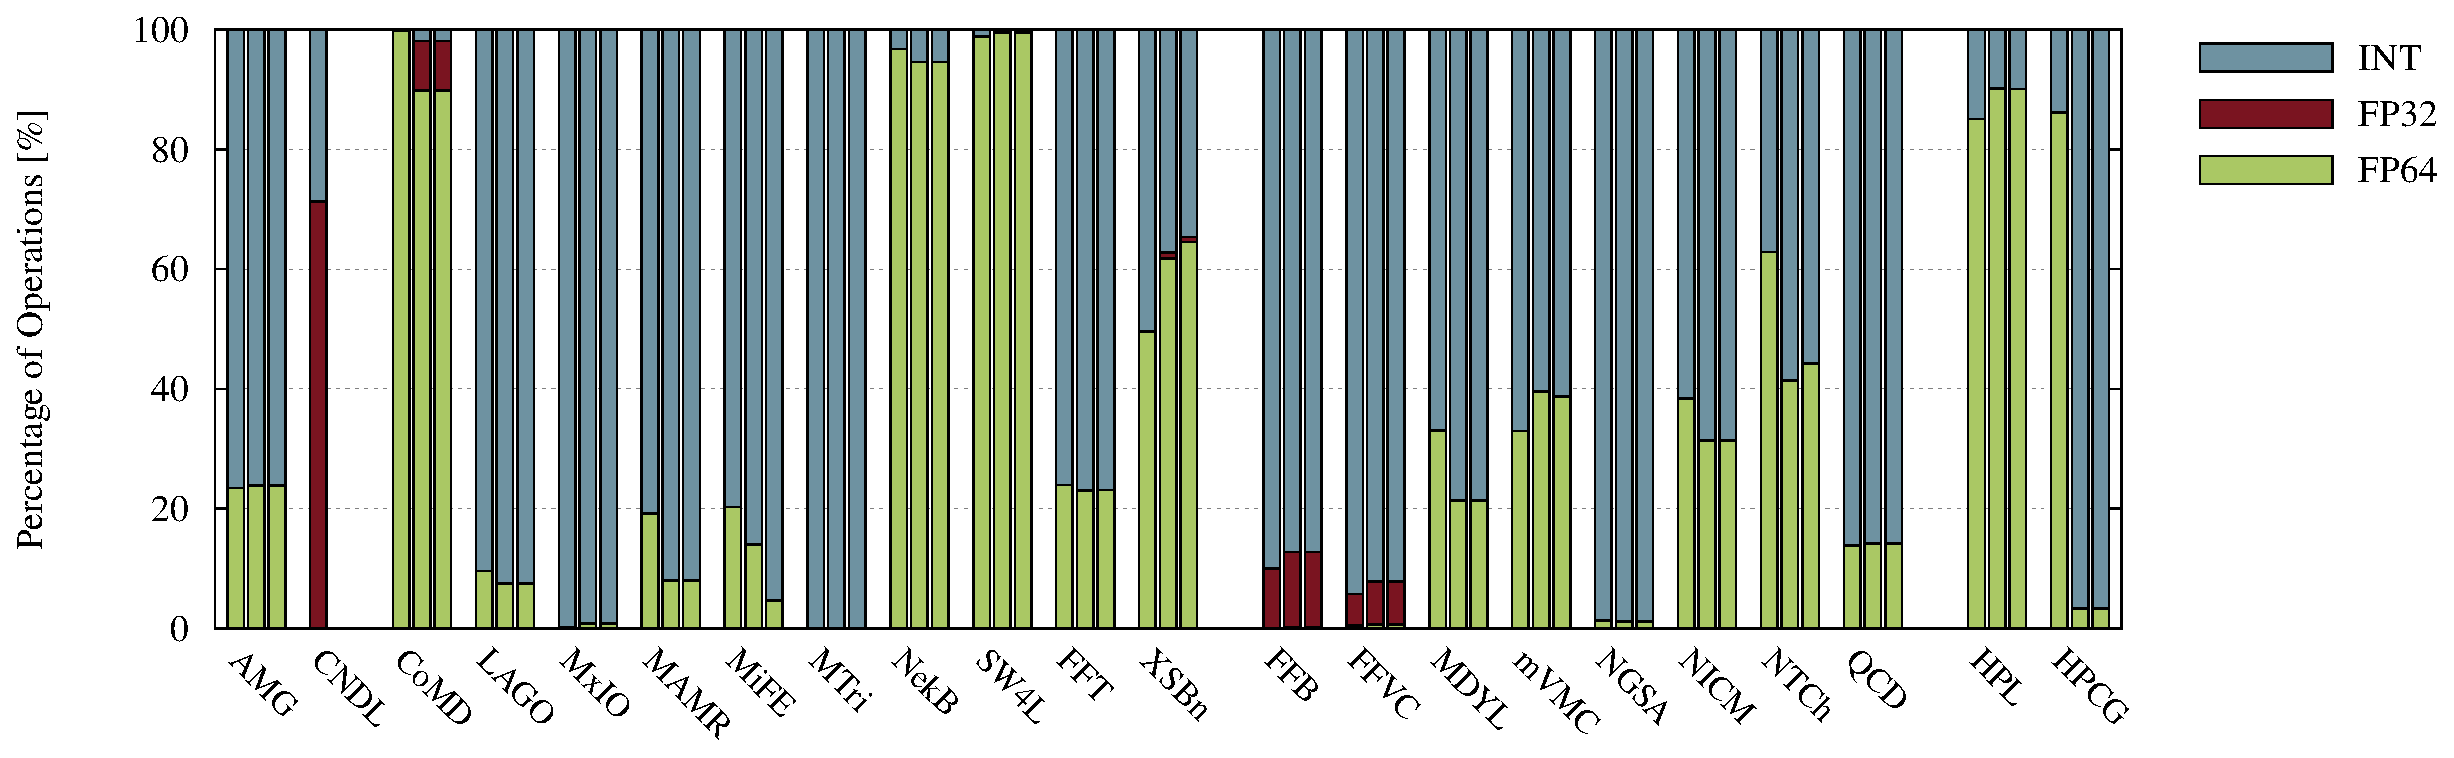
\includegraphics[width=\linewidth]{alu-fpu-ops}
    \caption{\label{fig:totalops} Ratio of Integer vs. single-precision FP vs. double-precision FP per proxy-app as counted by Intel's SDE; Per application: \textbf{Left bar = BDW, middle bar = KNL, right bar = KNM}; Missing bars for CANDLE due to SDE crashes on Xeon Phi; Proxy-app abbreviations acc. to Section~\ref{ssec:bm}}
\end{figure}
%
%\cJD{discuss the problem with int over-represented because of sde counting method}
The breakdown of total number of integer and single/double-precision floating point (FP) operations, as depicted in Figure~\ref{fig:totalops},
shows two rather unexpected trends. First, the number of proxy-apps relying on 32-bit FP instructions is four out of 22, which is surprisingly low, and furthermore, only one of them utilizes both 32-bit and 64-bit FP instructions.
Minor variances in integer to FP ratio between the architectures can likely be explained by the difference in
AVX vector length, quality of compiler optimization for each CPU, and execution/parallelization approach.
The second unexpected trend is the imbalance of integer to FP operations, i.e., 16 of 22 applications issue at least 50\%
integer operations. However, one has to keep in mind that Intel SDE output includes AVX vector instructions for integers, where
the granularity can be as low as 1-bit per operand (cf. 4 or \unit[8]{byte} per FP operand). Hence, the total integer operations
count might be slightly inflated.
Lastly, the results for HPCG show a big discrepancy between BDW and KNL/KNM. While the total FP operations count is similar,
the binary for KNL/KNM issues far more integer operations, see Table~\ref{table:rest} for details, and we are unaware of the reason.

\subsection{Floating-Point Operation/s and Time-to-Solution}\label{ssec:eval_flops}
%
\begin{figure}[tbp]
    \centering
    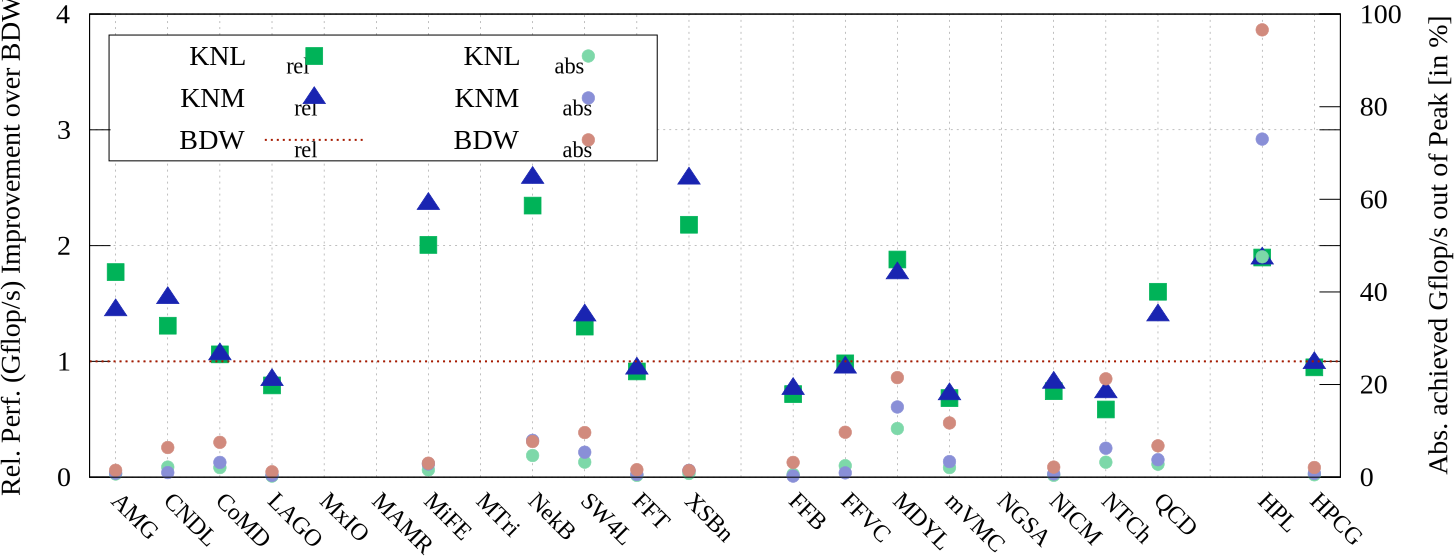
\includegraphics[width=\linewidth]{flops-rel}
    \caption{\label{fig:flops} Relative floating-point performance (FP32 and FP64 \unit[]{Gflop/s} accumulated) of KNL/KNM in comparison to dual-socket Broadwell-EP (see \textit{KEY}\textbf{\textsubscript{rel}}, left y-axis) and Absolute achieved \unit[]{Gflop/s} w.r.t dominant FP operations (cf. Fig.~\ref{fig:totalops}) in comparison to theoretical peak performance listed in Tab.~\ref{table:HW} (see \textit{KEY}\textbf{\textsubscript{abs}}, right y-axis); Due to missing SDE data for CANDLE, we assume the total number of FP operations is equivalent to BDW and divide by CANDLE's time-to-solution; Filtered proxy-apps with negligible FP operations: MxIO, MTri, and NGSA; Filtered out MiniAMR because of the strong-scaling issue described in Section~\ref{ssec:bmconf}; Proxy-app abbreviations acc. to Section~\ref{ssec:bm}}
    \vspace{-0.6em}
\end{figure}
\begin{comment}
\begin{figure}[tbp]
    \centering
    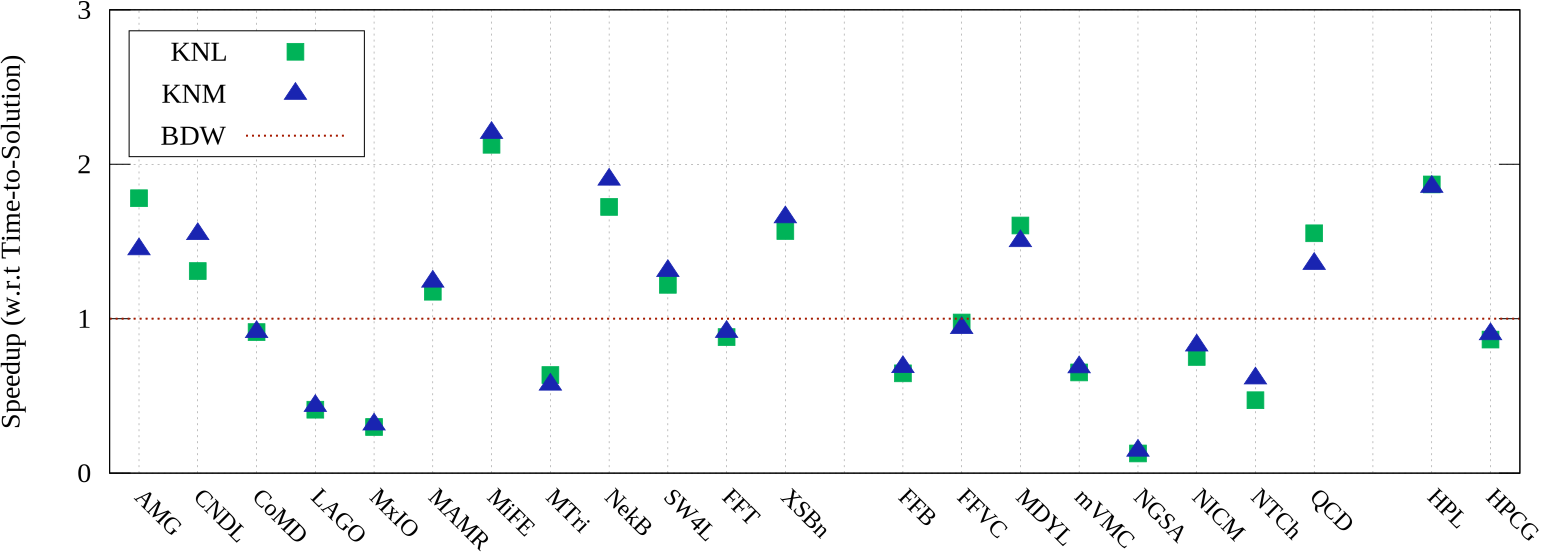
\includegraphics[width=\linewidth]{t2s-rel}
    \caption{\label{fig:t2s-knl-vs-knm} Speedup of KNM over KNL as baseline. MiniAMR included since the input is the same for both Phi\cJD{why call out MiniAMR?}; Proxy-app abbreviations acc. to Section~\ref{ssec:bm}}
\end{figure}
\end{comment}
%
Figure~\ref{fig:flops} shows the relative performance improvement of KNL/KNM over the dual-socket BDW node and the absolute achieved~\unit[]{Gflop/s} on each processor. It is important to note that all proxy-/mini-apps, with the exception of HPL, have less than~21.5\% (BDW), 10.5\% (KNL), and~15.1\%~(KNM) FP efficiency. Given that these applications are presumably optimized, and still achieve this low FP efficiency, implies a limited relevance of FP unit's availability. The figure shows that the majority of codes have comparable performance on KNM versus KNL. Notable mentions are: a)~CANDLE which benefits from VNNI units in mixed precision,
b)~MiFE, NekB, and XSBn which improve probably due to increased core count and KNM's higher CPU frequency,
%b)~NTChem as an outlier,
and c)~some memory-bound applications (i.e., AMG, HPCG, and MTri) which get slower supposedly due to the difference in peak throughput demonstrated in Figure~\ref{fig:memthru} in addition to the increased core count causing higher competition for bandwidth. 
%Finally, the results in figure~\ref{fig:t2s-knl-vs-knm} affirms that the FPU compute capacity, whether for fp64 or fp32, is marginally useful in the context of proxy/mini-apps.

\subsection{Memory Throughput of (MC-)DRAM}\label{ssec:eval_mem}
%
\begin{figure}[tbp]
    \centering
    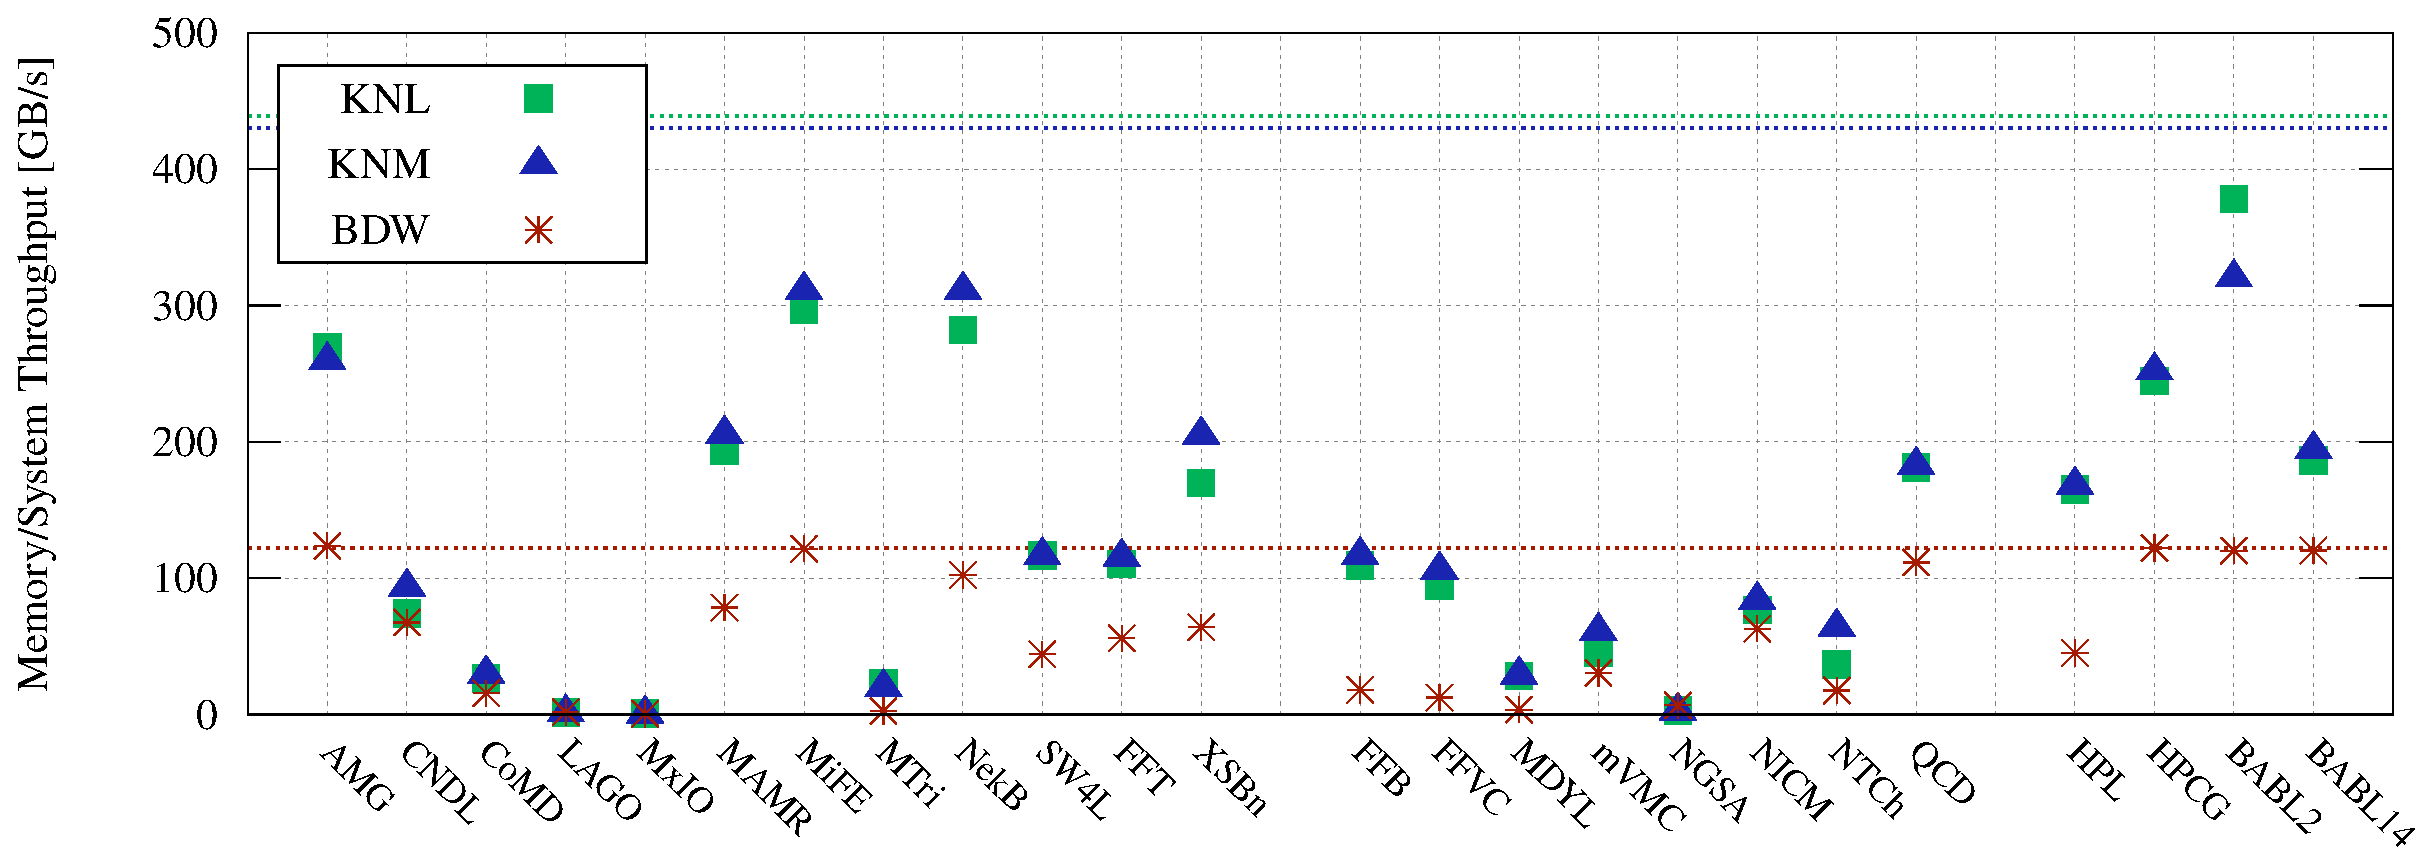
\includegraphics[width=\linewidth]{mem-throughput}
    \caption{\label{fig:memthru} Memory throughput (only DRAM for BDW, DRAM+MCDRAM for Phi) per proxy-app; Dotted lines indicate Triad stream bandwidth (flat mode, cf. Tab.~\ref{table:HW}); BabelStream for \unit[2]{GiB} (BABL2) and \unit[14]{GiB} (BABL14) vector length added (measured in cache mode); Proxy-app labels acc. to Section~\ref{ssec:bm}}
    \vspace{-0.6em}
\end{figure}
%
For the memory throughput measurements, shown in Figure~\ref{fig:memthru}, we use Intel's PCM tool to analyze DRAM and MCDRAM throughput.
Our measurements with BabelStream are included as well to demonstrate the maximum achievable bandwidth, see horizontal lines for MCDRAM
(in \textit{flat} mode), which is lower when the MCDRAM is used in \textit{cache} mode.
We still achieve~86\% on KNL and~75\% on KNM when the vectors fit into MCDRAM, but drop to slightly
higher than DRAM throughput (due to minor prefetching benefits) when the vectors do not fit (see BABL14 for \unit[14]{GiB} vectors).
This throughput advantage of the MCDRAM translates into a performance boost for six proxy-apps (AMG, MAMR, MiFE, NekB, XSBn, and QCD)
which heavily utilize the available bandwidth, see Figure~\ref{fig:memthru}, and which are memory-bound on our reference system.
This can easily be verified when comparing the time-to-solution for the kernels listed in Table~\ref{table:rest}.
Only HPCG cannot benefit from the higher bandwidth and, despite showing $\approx$2x throughput, the runtime drops by more than 10\%,
indicating a memory-latency issue of HPCG on KNL/KNM, which is one of the design goals for the benchmark~\cite{dongarra_new_2016}.
%
%\begin{figure}[tbp]
%    \centering
%    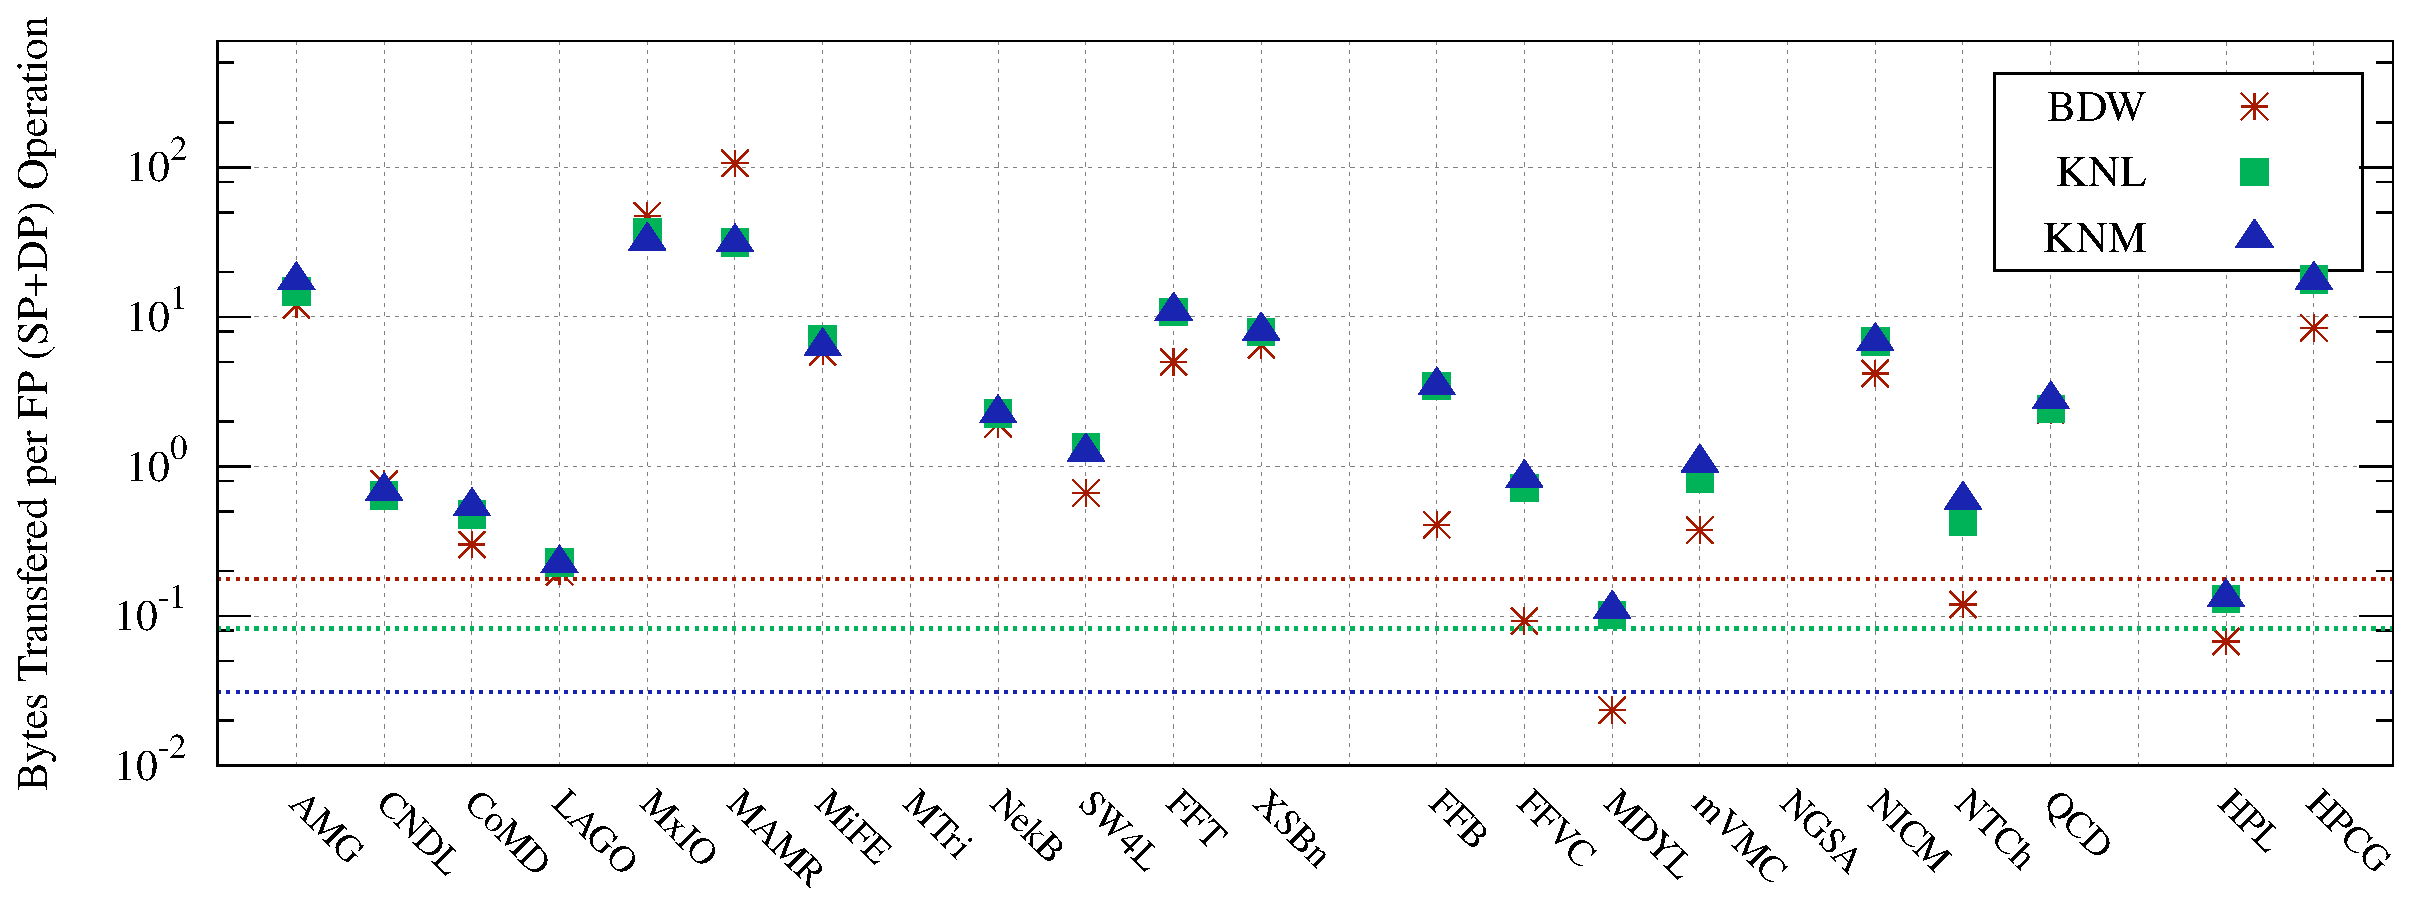
\includegraphics[width=\linewidth]{bpf-ratio}
%    \caption{\label{fig:bpfratio} \cJD{do we have space for bytes-per-flop?}}
%\end{figure}

\subsection{Frequency Scaling to Identify Compute-Boundedness}\label{ssec:eval_freq}
%
\begin{figure}[tbp]
    \centering
    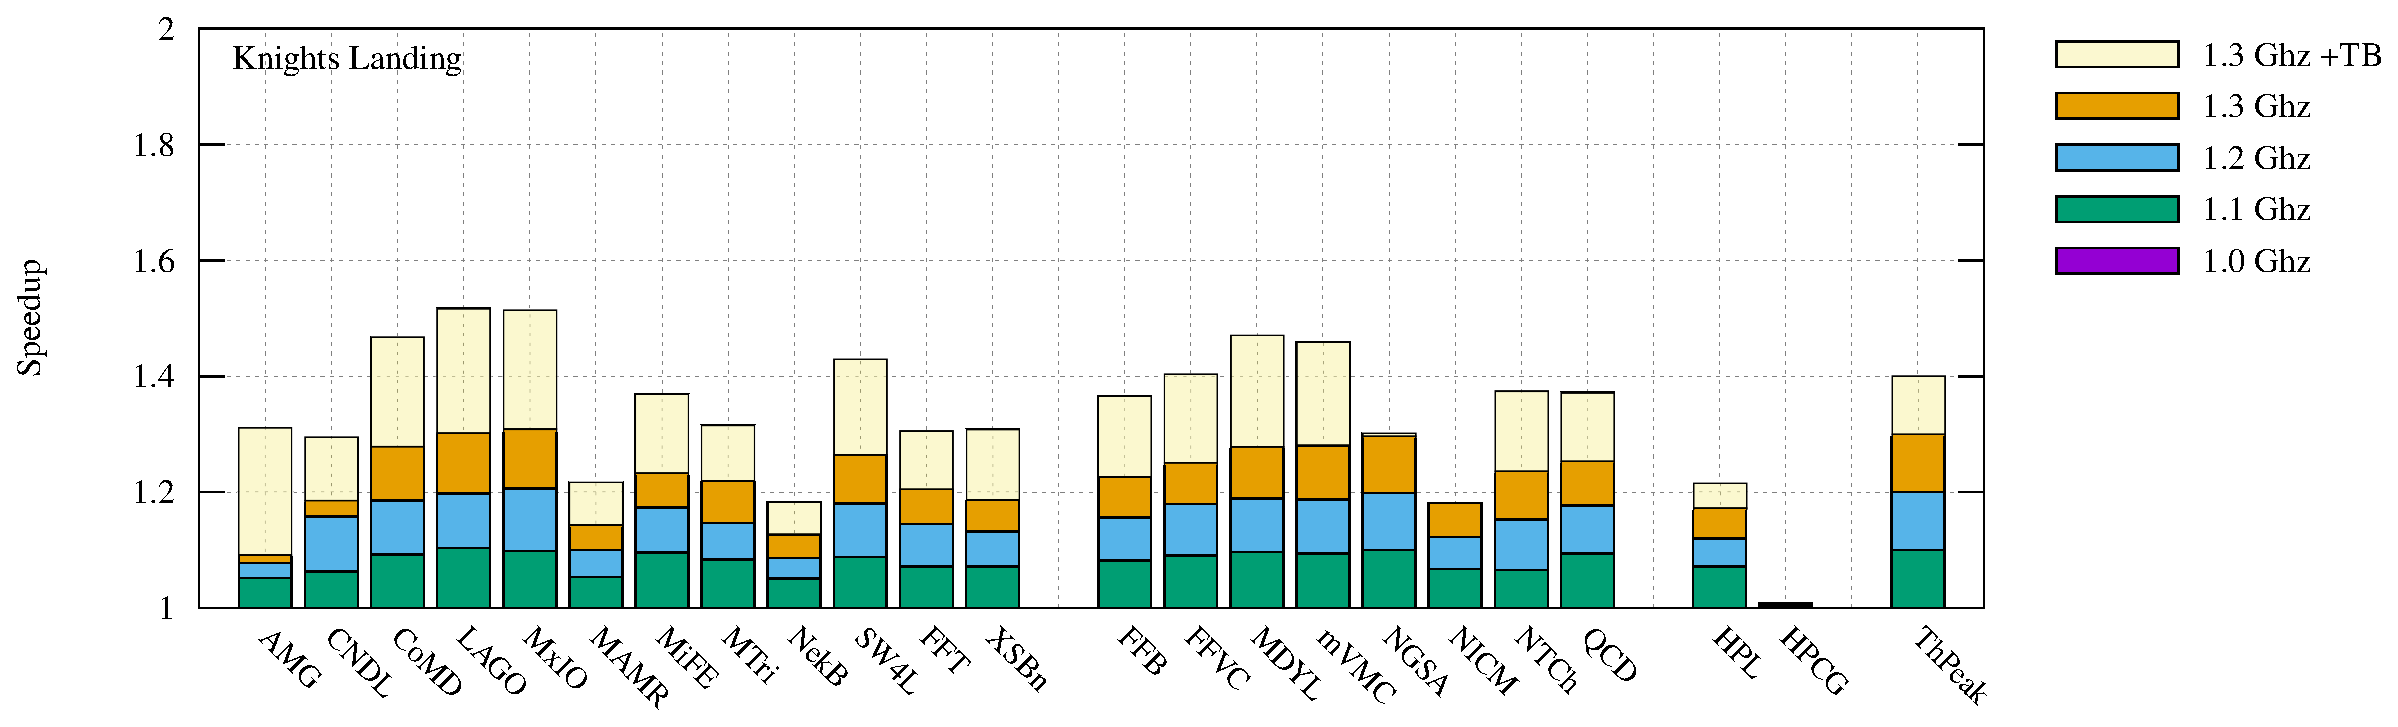
\includegraphics[width=\linewidth]{knl-freq}
    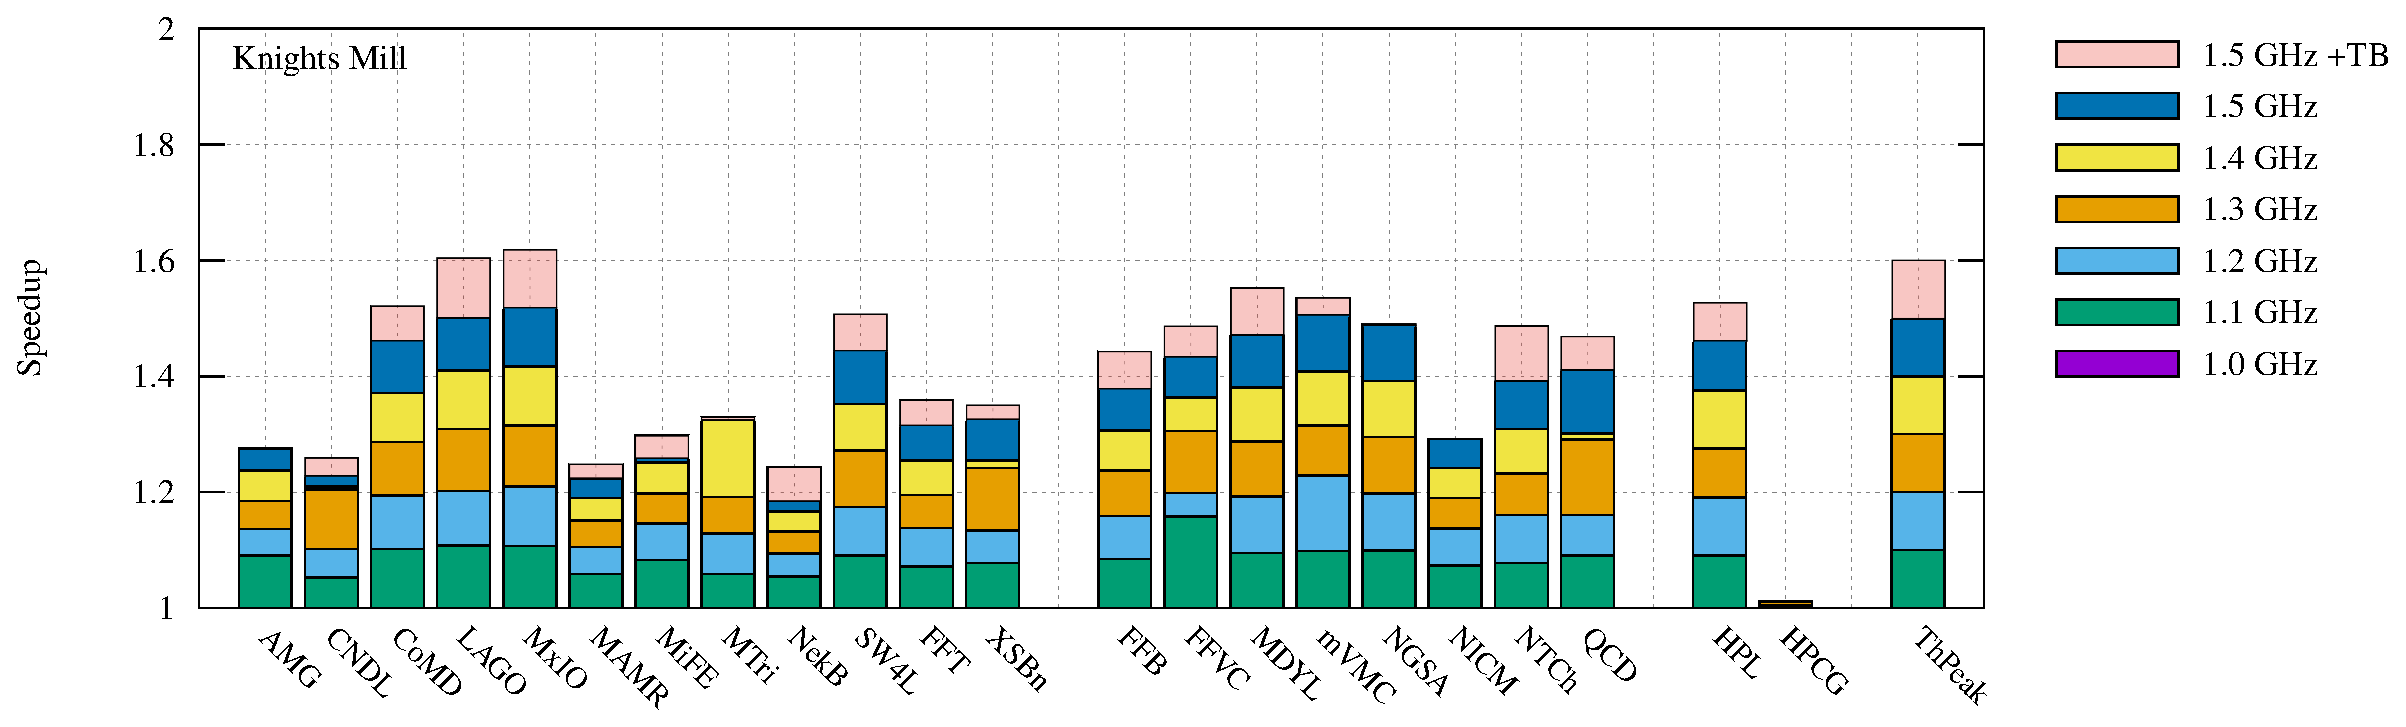
\includegraphics[width=\linewidth]{knm-freq}
    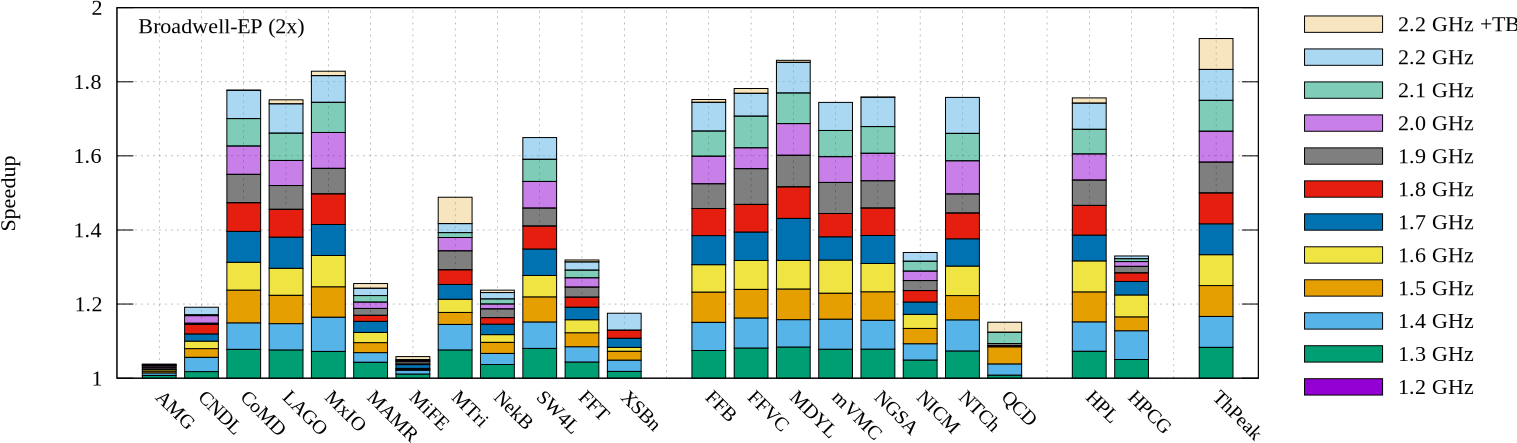
\includegraphics[width=\linewidth]{bdw-freq}
    \vspace*{-5mm}
    \caption{\label{fig:freq} Speedup obtained through increased CPU frequency (w.r.t baseline frequency of \unit[1.0]{GHz} on KNL/KNM and \unit[1.2]{GHz} on BDW); \textbf{Top plot: KNL, middle plot: KNL, bottom plot: BDW}; Theoretical peak (ThPeak): furthest right bar; Labels/abbreviations of proxy-apps according to Section~\ref{ssec:bm} and 'TB' = Turbo Boost is assumed to be \unit[100]{Mhz} across all cores}
    \vspace{-0.2em}
\end{figure}
%
\begin{figure}[tbp]
    \centering
    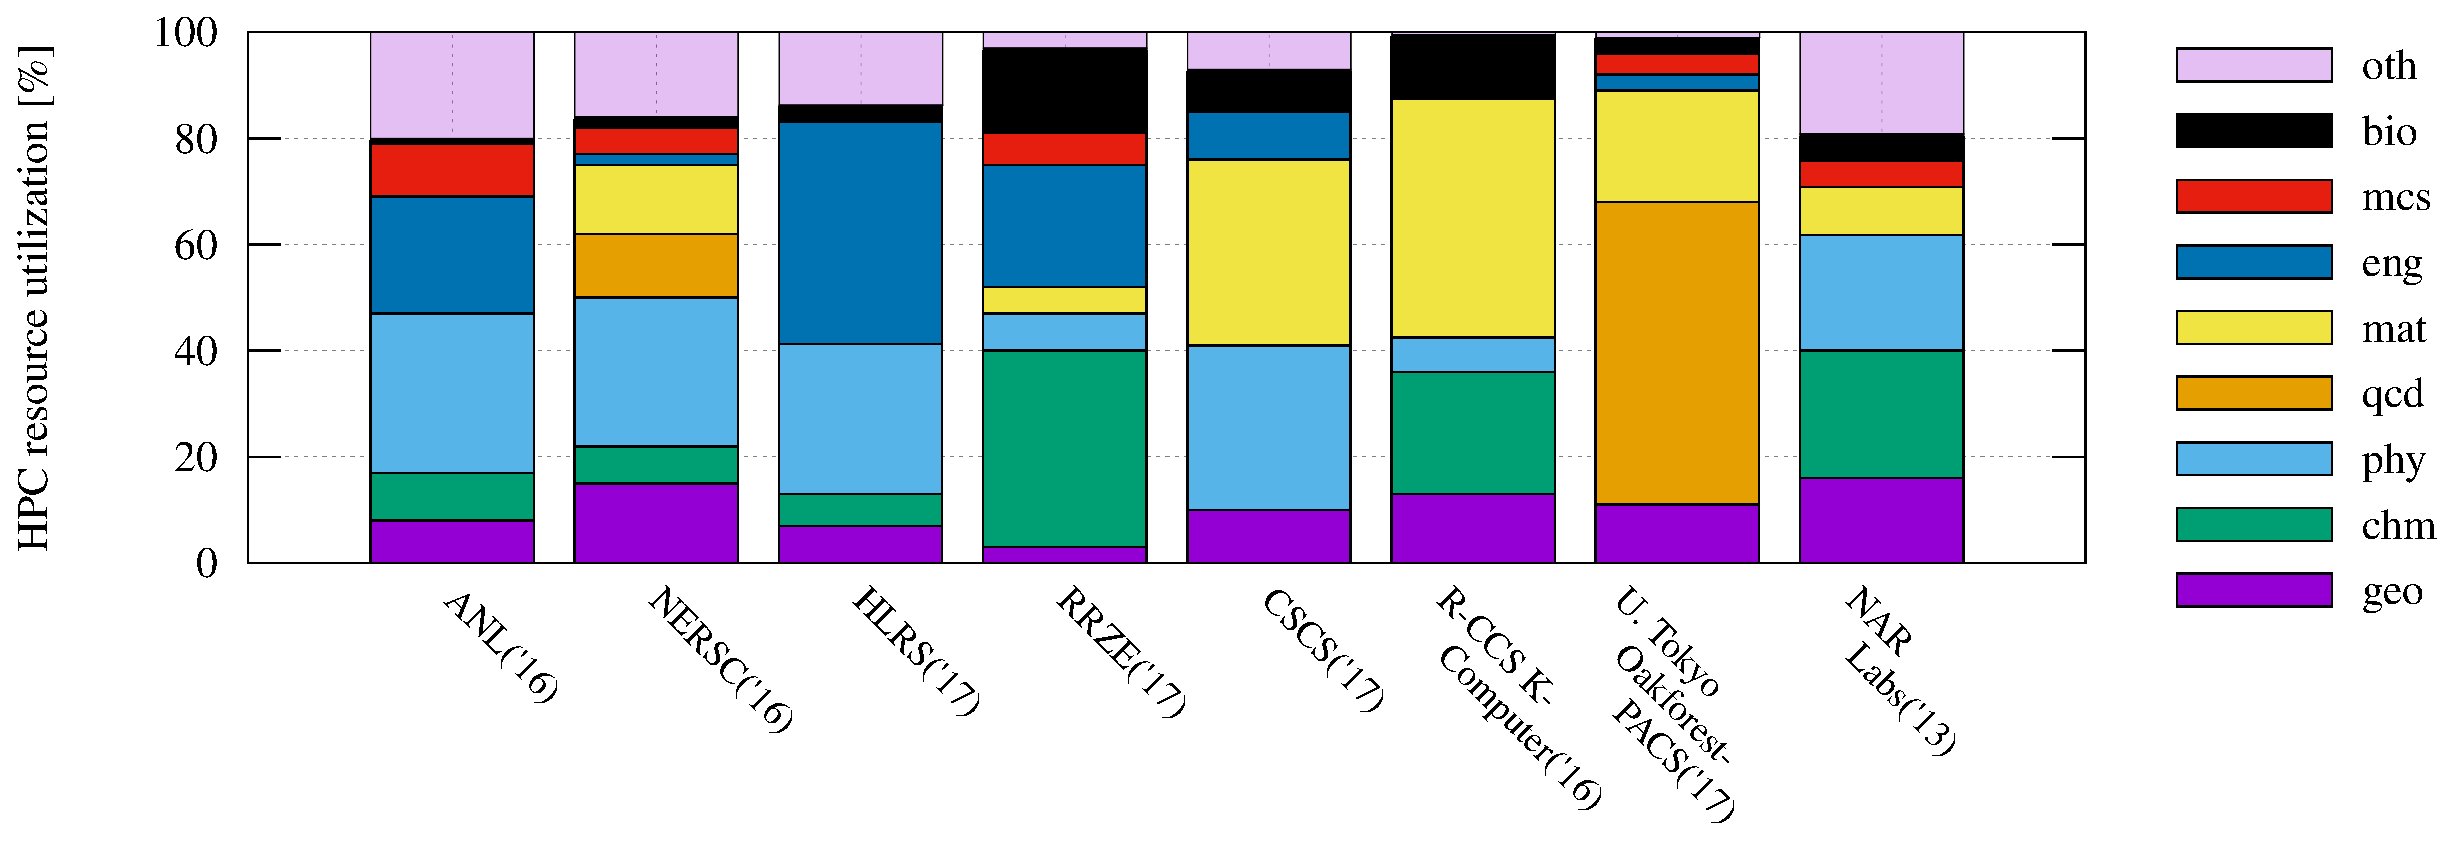
\includegraphics[width=\linewidth]{sys-util}
    \vspace*{-7mm}
    \caption{\label{fid:disc:breakdown} Annual HPC site/system utilization by domain; Labels acc. to Table~\ref{table:APP}: \texttt{geo} = Geo-/Earthscience, \texttt{chm} = Chemistry, \texttt{phy} = Physics, \texttt{qcd} = Lattice QCD, \texttt{mat} = Material Science/Engineering, \texttt{eng} = Engineering (Mechanics, CFD), \texttt{mcs} = Math/Computer Science, \texttt{bio} = Bioscience, \texttt{oth} = \textit{Other}}
    \vspace{-1em}
\end{figure}
%
For this test, we disable turbo boost and throttle core frequency, but keep uncore at maximum frequency which would otherwise negatively
affect the memory subsystem, to identify each application's dependency on ALU/FPU performance. The shown speedup (w.r.t time-to-solution) in Figure~\ref{fig:freq}
of each proxy-app is relative to the lowest CPU frequency on each architecture, and we include our \textit{performance} results
(cf. Section~\ref{ssec:bmconf}) with max.~frequency plus enabled turbo boost.

%\cJD{ecp on bdw mostly not compute bound, riken mostly compute bound}
%\cJD{hpl on knl doesnt scale while it does on knm, hence mill better balanced?!, hpcg doesnt scale at all on both}
%\cJD{on phi almost all apps benefit from turbo, on bwd non do so (except mini-tri}
While a benefit from enabled turbo boost on BDW is near invisible (except for MTri), the proxy-apps clearly reduce their
time-to-solution on KNL and KNM when the CPUs are allowed to turbo. Overall, the benchmarks seem to be less memory-bound
and more compute-bound, especially salient for AMG and MiniFE,  when moving to Xeon~Phi, indicating a clear benefit
from the much bigger/faster MCDRAM used as last-level cache and indicating a more balanced
(w.r.t bandwidth to \unit[]{flop/s} ratio) architecture.
%\cJD{phi compute to memory ratio (thru mcdram caching/speed) turns some clearly memory bound apps (from bdw) into
%semi-compute bound apps, see amg, minife for example}
However, the limited speedup for HPL on KNL clearly shows the CPU's abundance of FP64 units.
Here, the successor, Knights Mill, shows a better balance.
Another interesting observation is the inverse behavior of AMG and HPCG on our tested architecture.
Both benchmarks are supposed to be memory-bound, but the absence of signs of any scalability with frequency on Xeon~Phi
strengthens our hypothesis from Section~\ref{ssec:eval_mem} that HPCG is primarily memory-latency bound.

%\cJD{dd to verify IO scaling}
For I/O portions of an application, the Figure~\ref{fig:freq} reveals another observation, i.e., MACSio's write speed
scales with increased frequency. Since, MACSio performs only single figure \unit[]{GIop/s} and negligible
\unit[]{flop/s}, increasing the CPU's compute capabilities cannot explain the shown speedup.
Hence, our theory is: MACSio (and I/O in general) is bound by the Linux kernel, whose performance depends on CPU frequency.
Gu{\'e}rout et al. report similar findings~\cite{guerout_energy-aware_2013}, and we see equivalent behavior with 
a micro-benchmark (with Unix's \texttt{dd} command).


\subsection{Remaining Metrics}\label{ssec:eval_rest}
%
To disseminate the remaining results from our experiments, we 
attached Table~\ref{table:rest} to this paper, which can be utilized for
further analysis, and which contains some interesting data points.
For example, the power measurements for CANDLE, which is just slightly
higher than when running MACSio, indicate that Intel's MKL-DNN (used
underneath to compute on the FP16 VNNI units) does not
fully utilize the CPU's potential. Furthermore, the L2 hit rate on both
Xeon Phi is considerably higher than on our reference
hardware, indicating improvements in the hardware prefetcher and are presumably
a direct effect of the high-bandwidth MCDRAM in \textit{cache} mode.

\begin{comment}
\begin{table*}[tbp]
    \caption{\label{table:rest} Application configuration and measured metrics; Missing data for CANDLE due to SDE crashes on Phi; Measurements indicate CANDLE/MKL-DNN ignores OpenMP settings and tries to utilize full chip $\rightarrow$ listed in italic; Label explanation: t2sol = time-to-solution (kernel), Gop (D $|$ S $|$ I) = Giga operations (FP64 $|$ FP32 $|$ Integer), SIMDi/cyc = SIMD instructions per cycle, FPAIp[R $|$ W] = FP Arithmetic instructions per memory [read $|$ write], [B $|$ M]Bd = [Back-end $|$ Memory] Bound (see~\cite{sobhee_intel_2018} for details), L2h = L2 cache hit rate, LLh = Last level cache hit rate (L3 for BDW, MCDRAM for KNL/KNM), Gbra/s = Giga branches/s}%\cJD{highlight important?}}
    \centering\scriptsize
    \begin{tabular}{|l|r|r|r|r|r|r|r|c|r|r|r|r|}
        \hline \hC
        \tH{\textbf{KNL}} & \tH{\#MPI} & \tH{\#OMP} & \tH{t2sol [\unit[]{s}]} & \tH{\#Gop (D)} & \tH{\#Gop (S)} & \tH{\#Gop (I)} &  \tH{Power [\unit[]{W}]} & \tH{\#SIMDi/cyc} & \tH{BBd [\%]} & \tH{L2h [\%]} & \tH{LLh [\%]} & \tH{Gbra/s} \\ \hline
        AMG	        &	1	&	128	&	6.057	&	110.271	&	0	&	352.640	&	202.16	&	0.063	&	77.3	&	93	&    74.6	&	7.310	\\ \hline \rC
        CANDLE	    &	1	&	\textit{32}	&	59.796	&	\textit{N/A}	&	\textit{N/A}	&	\textit{N/A}	&	143.79	&	0.105	&	67.4	&	86	&    89.7	&	\textit{N/A}	\\ \hline
        CoMD	    &	32	&	8	&	3.199	&	161.691	&	14.842	&	3.476	&	189.24	&	0.077	&	81.0	&	85	&    99.4	&	11.551	\\ \hline \rC
        Laghos	    &	64	&	4	&	13.508	&	85.547	&	0.422	&	1055.977	&	143.84	&	0.021	&	23.7	&	98	&    99.7	&	7.839	\\ \hline
        MACSio	    &	64	&	1	&	35.110	&	0.613	&	0.007	&	77.884	&	140.02	&	0.002	&	52.8	&	98	&    98.6	&	18.115	\\ \hline \rC
        miniAMR	    &	128	&	1	&	47.150	&	291.536	&	0.014	&	3358.569	&	153.44	&	0.009	&	75.9	&	71	&    97.6	&	5.023	\\ \hline
        miniFE	    &	1	&	256	&	0.694	&	28.961	&	0	&	177.704	&	221.69	&	0.022	&	81.8	&	93	&    93.6	&	10.930	\\ \hline \rC
        miniTri	    &	1	&	128	&	8.630	&	0	&	0	&	118.261	&	131.49	&	0.001	&	81.9	&	66	&    99.5	&	4.531	\\ \hline
        Nekbone	    &	128	&	1	&	3.290	&	410.361	&	0	&	23.371	&	221.48	&	0.050	&	76.5	&	87	&    97.6	&	6.125	\\ \hline \rC
        SW4lite	    &	64	&	4	&	1.686	&	145.938	&	0	&	0.761	&	214.57	&	0.096	&	80.6	&	95	&    98.4	&	2.218	\\ \hline
        SWFFT	    &	128	&	1	&	1.235	&	12.688	&	0.005	&	42.509	&	174.12	&	0.029	&	76.7	&	83	&    98.6	&	20.905	\\ \hline \rC
        XSBench	    &	1	&	256	&	1.290	&	27.283	&	0.417	&	16.441	&	192.46	&	0.041	&	93.7	&	22	&    99.5	&	2.629	\\ \hline\hline
        FFB	        &	64	&	2	&	8.244	&	2.300	&	258.561	&	1785.716	&	179.55	&	0.159	&	38.4	&	89	&    99.7	&	2.717	\\ \hline \rC
        FFVC	    &	1	&	64	&	13.009	&	134.589	&	1579.917	&	20174.483	&	180.58	&	0.169	&	36.0	&	95	&    99.7	&	4.415	\\ \hline
        mVMC	    &	32	&	6	&	20.679	&	1141.865	&	1.345	&	1746.001	&	180.98	&	0.036	&	81.9	&	91	&    98.9	&	6.073	\\ \hline \rC
        MODYLAS	    &	64	&	4	&	22.514	&	6287.279	&	2.063	&	23104.728	&	206.98	&	0.072	&	80.4	&	97	&    95.7	&	7.742	\\ \hline
        NGSA	    &	4	&	32	&	829.675	&	0.826	&	0.023	&	69.117	&	97.91	&	0.002	&	51.9	&	71	&    95.9	&	1.050	\\ \hline \rC
        NICAM	    &	10	&	15	&	37.802	&	422.504	&	0.066	&	925.228	&	119.46	&	0.193	&	67.8	&	92	&    99.2	&	0.231	\\ \hline
        NTChem	    &	16	&	8	&	18.985	&	1629.210	&	0.627	&	2303.804	&	167.13	&	0.060	&	64.4	&	91	&    99.2	&	5.429	\\ \hline \rC
        QCD	        &	1	&	128	&	8.437	&	631.522	&	0	&	3823.335	&	215.67	&	0.220	&	69.4	&	88	&    95.4	&	1.151	\\ \hline\hline
        HPCG	    &	96	&	1	&	44.612	&	612.799	&	0	&	17530.136	&	181.69	&	0.023	&	86.1	&	91	&    45.7	&	1.446	\\ \hline \rC
        HPL	        &	64	&	1	&	145.400	&	184191.774	&	0.015	&	20226.567	&	221.13	&	0.374	&	52.3	&	93	&    87.9	&	1.232	\\ \hline
        \hline \hC
        \tH{\textbf{KNM}} & \tH{\#MPI} & \tH{\#OMP} & \tH{t2sol [\unit[]{s}]} & \tH{\#Gop (D)} & \tH{\#Gop (S)} & \tH{\#Gop (I)} &  \tH{Power [\unit[]{W}]} & \tH{\#SIMDi/cyc} & \tH{BBd [\%]} & \tH{L2h [\%]} & \tH{LLh [\%]} & \tH{Gbra/s} \\ \hline
        AMG	        &	1	&	128	&	7.434	&	110.271	&	0	&	352.639	&	202.52	&	0.062	&	75.4	&	94	&   73.3	&	6.392	\\ \hline \rC
        CANDLE	    &	1	&	\textit{144}	&	50.527	&	\textit{N/A}	&	\textit{N/A}	&	\textit{N/A}	&	153.69	&	0.040	&	82.4	&	92	&	90.9	&	\textit{N/A}	\\ \hline
        CoMD	    &	72	&	2	&	3.194	&	161.842	&	14.880	&	3.479	&	196.64	&	0.177	&	67.5	&	86	&	99.1	&	11.546	\\ \hline \rC
        Laghos	    &	64	&	4	&	12.725	&	85.383	&	0.422	&	1056.141	&	139.33	&	0.023	&	25.1	&	98	&	99.8	&	8.345	\\ \hline
        MACSio	    &	64	&	1	&	33.236	&	0.613	&	0.007	&	77.884	&	135.48	&	0.002	&	53.8	&	98	&	98.2	&	19.206	\\ \hline \rC
        miniAMR	    &	128	&	1	&	44.653	&	291.536	&	0.014	&	3358.570	&	177.31	&	0.009	&	75.3	&	71	&	97.3	&	5.337	\\ \hline
        miniFE	    &	72	&	1	&	0.669	&	32.892	&	0	&	669.371	&	210.18	&	0.097	&	55.6	&	60	&	98.3	&	7.393	\\ \hline \rC
        miniTri	    &	1	&	128	&	9.545	&	0	&	0	&	118.262	&	122.02	&	0	&	80.9	&	68	&	99.6	&	4.102	\\ \hline
        Nekbone	    &	144	&	1	&	2.984	&	410.381	&	0	&	23.470	&	233.46	&	0.040	&	76.1	&	87	&	96.6	&	6.494	\\ \hline \rC
        SW4lite	    &	72	&	4	&	1.569	&	146.048	&	0	&	0.764	&	228.01	&	0.090	&	81.3	&	96	&	97.8	&	2.753	\\ \hline
        SWFFT	    &	128	&	1	&	1.189	&	12.555	&	0.005	&	41.732	&	172.66	&	0.026	&	77.2	&	83	&	98.5	&	21.990	\\ \hline \rC
        XSBench	    &	1	&	288	&	1.220	&	30.603	&	0.417	&	16.440	&	197.16	&	0.038	&	91.5	&	22	&	98.5	&	2.783	\\ \hline\hline
        FFB	        &	64	&	2	&	7.750	&	2.300	&	258.565	&	1785.712	&	178.72	&	0.171	&	38.6	&	89	&	99.7	&	2.886	\\ \hline \rC
        FFVC	    &	1	&	72	&	13.497	&	134.589	&	1579.917	&	20174.587	&	182.05	&	0.162	&	55.2	&	94	&	99.9	&	5.055	\\ \hline
        mVMC	    &	72	&	4	&	19.659	&	1140.670	&	1.347	&	1802.663	&	197.64	&	0.012	&	76.0	&	91	&	98.5	&	8.869	\\ \hline \rC
        MODYLAS	    &	64	&	4	&	24.026	&	6287.279	&	2.063	&	23104.728	&	217.47	&	0.062	&	80.0	&	97	&	95.6	&	7.153	\\ \hline
        NGSA	    &	4	&	18	&	724.546	&	0.826	&	0.023	&	69.300	&	88.67	&	0.002	&	39.5	&	68	&	94.9	&	1.138	\\ \hline \rC
        NICAM	    &	10	&	7	&	34.380	&	422.504	&	0.066	&	925.229	&	113.88	&	0.208	&	68.2	&	92	&	99.1	&	0.248	\\ \hline
        NTChem	    &	72	&	2	&	14.606	&	1575.310	&	0.623	&	1985.255	&	176.51	&	0.066	&	59.0	&	90	&	98.4	&	7.038	\\ \hline \rC
        QCD	        &	1	&	144	&	9.662	&	631.522	&	0	&	3823.337	&	200.86	&	0.175	&	72.6	&	88	&	95.9	&	2.121	\\ \hline\hline
        HPCG	    &	64	&	1	&	42.865	&	612.605	&	0	&	17532.326	&	174.58	&	0.041	&	86.5	&	95	&   42.9	&	2.878	\\ \hline \rC
        HPL	        &	72	&	1	&	146.562	&	184893.073	&	0.016	&	20414.548	&	263.59	&	0.351	&	57.0	&	92	&   87.0	&	1.885	\\ \hline
        \hline \hC
        \tH{\textbf{BDW}} & \tH{\#MPI} & \tH{\#OMP} & \tH{t2sol [\unit[]{s}]} & \tH{\#Gop (D)} & \tH{\#Gop (S)} & \tH{\#Gop (I)} & \tH{Power [\unit[]{W}]} & \tH{FPAIp[R : W]} & \textcolor{white}{MBd [\%]} & \tH{L2h [\%]} & \tH{LLh [\%]} & \tH{Gbra/s} \\ \hline
        AMG	        &	8	&	6	&	10.780	&	110.810	&	0	&	362.209	&	152.21	&	0.361 : 5.516	&	44.8	&	21		&	17  &	4.354	\\ \hline \rC
        CANDLE	    &	1	&	\textit{12}	&	78.240	&	0.012	&	6918.340	&	2783.532	&	132.38	&	1.078 : 2.800	&	26.7	&	23		&    11	&	1.242	\\ \hline
        CoMD	    &	48	&	1	&	2.921	&	152.022	&	0	&	0.205	&	133.17	&	0.845 : 6.615	&	1.5		&	15		&    15	&	11.391	\\ \hline \rC
        Laghos	    &	24	&	1	&	5.5472	&	44.534	&	0	&	421.465	&	126.51	&	0.184 : 0.476	&	13.2	&	81		&    56	&	16.808	\\ \hline
        MACSio	    &	4	&	1	&	10.498	&	0.070	&	0	&	72.582	&	89.3	&	0 : 0	&	0.8		&	48		&    59	&	3.274	\\ \hline \rC
        miniAMR	    &	96	&	1	&	55.386	&	40.816	&	0	&	172.317	&	133.29	&	0.059 : 0.311	&	55.1	&	24		&    23	&	4.013	\\ \hline
        miniFE	    &	24	&	1	&	1.475	&	30.693	&	0	&	120.715	&	152.77	&	0.311 : 5.454	&	55.2	&	15		&    12	&	4.699	\\ \hline \rC
        miniTri	    &	1	&	48	&	5.478	&	0	&	0	&	118.178	&	112.61	&	0 : 0	&	34.0	&	47		&	90    &	7.106	\\ \hline
        Nekbone	    &	96	&	1	&	5.671	&	301.559	&	0	&	10.139	&	154.74	&	0.593 : 2.431	&	36.9	&	36		&	24    &	3.915	\\ \hline \rC
        SW4lite	    &	24	&	2	&	2.056	&	136.835	&	0	&	1.585	&	146.65	&	1.044 : 4.580	&	9.1		&	75		&    18	&	1.112	\\ \hline
        SWFFT	    &	32	&	1	&	1.088	&	12.239	&	0	&	38.782	&	134.55	&	0.117 : 0.675	&	28.3	&	23		&    32	&	20.932	\\ \hline \rC
        XSBench	    &	1	&	96	&	2.022	&	19.921	&	0	&	20.280	&	132.25	&	0.807 : 3.847	&	71.7	&	5		&    18	&	1.653	\\ \hline\hline
        FFB	        &	24	&	1	&	5.327	&	1.300	&	233.640	&	2116.421	&	144.35	&	0.635 : 2.200	&	21.3	&	79		&    33	&	3.723	\\ \hline \rC
        FFVC	    &	12	&	4	&	12.691	&	127.322	&	1573.782	&	27857.376	&	151.85	&	0.481 : 2.844	&	3.3		&	84		&    57	&	9.045	\\ \hline
        mVMC	    &	24	&	2	&	13.489	&	1092.394	&	0	&	2224.092	&	152.28	&	0.601 : 2.456	&	12.0	&	36		&    24	&	10.170	\\ \hline \rC
        MODYLAS	    &	16	&	3	&	36.101	&	5363.366	&	0	&	10888.745	&	135.75	&	0.875 : 8.736	&	8.1		&	60		&    31	&	5.385	\\ \hline
        NGSA	    &	12	&	4	&	105.879	&	0.826	&	0.023	&	64.249	&	107.15	&	0.002 : 0.006	&	6.5		&	21		&    36	&	8.566	\\ \hline \rC
        NICAM	    &	10	&	6	&	28.449	&	428.282	&	0.003	&	687.852	&	118.32	&	0.540 : 3.732	&	49.6	&	27		&    19	&	0.585	\\ \hline
        NTChem	    &	24	&	1	&	8.963	&	1315.509	&	0	&	778.829	&	141.3	&	0.867 : 4.931	&	9.4		&	56		&    39	&	10.173	\\ \hline \rC
        QCD	        &	1	&	24	&	13.102	&	612.303	&	0	&	3817.944	&	153.2	&	1.152 : 4.542	&	45.2	&	27		&    24	&	0.368	\\ \hline\hline
        HPCG	    &	2	&	24	&	38.595	&	559.046	&	0	&	90.171	&	166.18	&	0.143 : 0.628	&	11.3	&	34		&    23		&	10.928	\\ \hline \rC
        HPL	        &	24	&	1	&	271.794	&	181484.240	&	0	&	31919.479	&	189.37	&	\,~~2.280 : 122.693	&	3.9		&	10		&    3    	&	2.147	\\ \hline
    \end{tabular}
\end{table*}
\end{comment}